\section{Interface Descriptions}
While it may seem far removed from the core programming aspect of software engineering, the design of a good user interface is key to the success of any system. Indeed, Douglas Bell (1987) went so far as to claim that the user interface is the ``yardstick by which a system is judged'', and certainly it plays a crucial role in attracting users to the software.

This section will describe what factors are taken into consideration in the design of the interface for the Fortitude application, and how the final product will be suitable, appealing and fulfil the criteria set forth in the requirements document (23 Cats, 2012).

\subsection{Design Methodology}

\begin{wrapfigure}{l}{0.25\textwidth}
	\vspace{-20pt}
	\begin{center}
	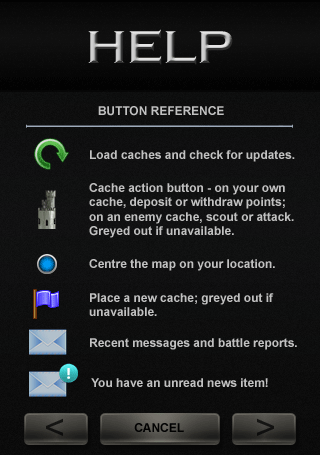
\includegraphics[width=0.25\textwidth]{images/help_mockup}
	\caption{Button reference in the help section.}
	\end{center}
	\vspace{20pt}
\end{wrapfigure}

While designing the interface, it was important at all times to consider ease of use for users of various levels of familiarity with the system. Our domain analysis had highlighted the importance of intuitiveness in a system and of required functions being easily accessible (23 Cats, 2012:5-7); for this reason we have tried at all times to make the interface clear, and have also included a help screen should the user ever require it (see fig 2.1). Bell (1987) highlights the role of a well designed user interface in reducing errors, and to this end several of the features of our app were tested on potential users during development. In particular, it had originally been decided to disable the android back button within the app to give us greater control over which screens the user could access at any point in time. However, our users found the lack of a back button difficult to get used to, and so its functionality has been incorporated into the application wherever possible.

\begin{wrapfigure}{r}{0.25\textwidth}
	\vspace{-20pt}
	\begin{center}
	
\includegraphics[width=0.2\textwidth]{images/flags_greye}
	\caption{The available (left) and unavailable (right) place cache button.}
	\end{center}
	\vspace{-20pt}
\end{wrapfigure}

To further the ease of use of the Fortitude Application, buttons which perform a specific action will be greyed out when the action is not available. These include, for example, the ‘place cache’ button which would be greyed out if the user was too close to an existing cache, shown right in fig 2.2. The greyed out flag would perform no action if it was clicked on.

Every screen on the application has been designed to satisfy non-functional requirement 5.3.7: Interface Style Uniformity by using a consistent colour scheme and placement of buttons and headers. The colour scheme has been chosen to be silver or white on black, as the monochrome black and white is easy for all people to read, including those who are colour blind.

Non-functional requirement 5.3.9: Interface Feedback Delay requires that the app provide a fast response to user input; this has been achieved by the use of separate images for on-press actions, as shown below in fig 2.3. The change in luminosity of the buttons when pressed ensures the user is aware that the system has received their request.

\begin{figure}
	\vspace{-20pt}
	\begin{center}
	
\includegraphics[width=0.2\textwidth]{images/news_icons}
	\caption{An inactive button (left) and an active button (right).}
	\end{center}
	\vspace{-10pt}
\end{figure}

\subsection{Fortitude-game.co.uk Website}

The website is a supporting feature to the Fortitude application. With its larger dimensions and lack of battery and data restraints, the website can incorporate much of the functionality that is not feasible to include on the app, such as 5.3.6: Activity Recording. This serves to make the app simpler and therefore more user friendly without compromising the scope of the system.

The website is also the chosen interface for administrators to use to interact with the app as specified by a variety of requirements including 5.1.3: Administrator Accounts. The web interface provides an easy to access alternative to bespoke software and is not device dependant in the way that the app itself is; as administrators may not have an Android device, no administrator actions are incorporated into the app itself.

\begin{figure}
	\vspace{-20pt}
	
\includegraphics[width=0.9\textwidth]{images/website_header_background}
	\caption{The header image, an example of the more complex graphics used in the website. The white bordered box will hold the navigation.}
	\vspace{-10pt}
\end{figure}

Requirement 5.4.8: Website Application Style Uniformity requires the overall design of the website to match that of the application. This has been achieved with the use of the same white on black colour scheme and recurring details such as Fortitude logo of two flags flying over a castle tower and the navigation menu of the website echoing the message box of the app. However, the simplicity of design used on the app has been expanded upon in the website with the addition of more dramatic imagery (see fig 2.4). This makes the website visually appealing without sacrificing ease of use as would be the case should such graphics be incorporated into the app.

\begin{wrapfigure}{r}{0.25\textwidth}
	\vspace{-20pt}
	\begin{center}
	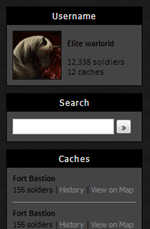
\includegraphics[width=0.2\textwidth]{images/sidebar_modules}
	\caption{Examples of the individual ‘modules’ that comprise the website (in this instance, the sidebar).}
	\end{center}
	\vspace{-20pt}
\end{wrapfigure}

Commonly accessed areas of the website, such as the sidebar and the home page, are organised into modules, as in fig 2.5, making information quickly and easily identifiable. It also provides an excellent template for adaptation; though out of scope for this project, users could in future personalise their interaction with the website through selecting which of these ‘modules’ to display on the side bar and home page. 

\begin{wrapfigure}{l}{0.25\textwidth}
	\vspace{-20pt}
	\begin{center}
	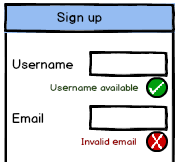
\includegraphics[width=0.2\textwidth]{images/sign_up_wireframe}
	\caption{Wireframe showing user feedback when creating an account.}
	\end{center}
	\vspace{-20pt}
\end{wrapfigure}

As in the application, the fortitude-game.co.uk website provides feedback in order to increase the efficiency with which the user can interact with the website and to reduce errors. This feedback can be in the form of data validation, such as in fig 2.6, or providing  a loading message while a section of the page loads. For more critical data entry, such as an administrator creating a new cache, the user is presented with a summary page of the information they have entered and must confirm it is correct before the new data is stored. This provides confirmation of the action as well as giving the user the chance to reduce errors, a key requirement of a well designed user interface.

The website also provides feedback if an error occurs – the most common is anticipated to be that the user has javascript disabled, which will cause every javascript dependent element of the site to be replaced with a placeholder informing the user that javascript is required and of the correct size and shape to avoid disturbing the rest of the website layout.

\section{Process Descriptions}
\subsection{Opening the application}

\begin{wrapfigure}{l}{0.5\textwidth}
	\vspace{-20pt}
	\begin{center}
	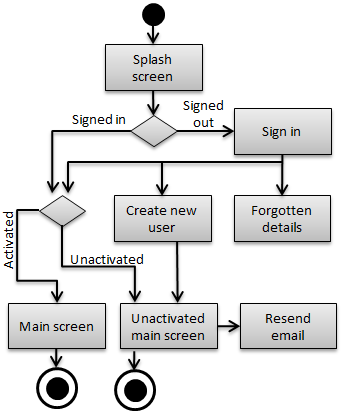
\includegraphics[width=0.5\textwidth]{images/opening_app}
	\caption{Screen map for the process of opening the app.}
	\end{center}
	\vspace{-20pt}
\end{wrapfigure}

The process of the user opening the application is designed to be quick and efficient. To this end, the user will be taken straight to the main screen from the splash screen if they are already signed in to the application.

The choice between the main and unactivated main screens reflects functional requirement 5.1.2: Account activation, whereby users who have not activated their accounts are given limited functionality while using the application. The screen to create a new user leads directly to this unactivated main screen; once the user has activated their account through the verification email sent to them on creating the account, they will be taken to the main screen the next time they open the app. As per functional requirement 5.1.4: Resend activation email, the user is given the opportunity from the unactivated main screen to request a second email be sent should they have not received the first.

\subsection{Performing key game actions}

\begin{wrapfigure}{l}{0.5\textwidth}
	\vspace{-20pt}
	\begin{center}
	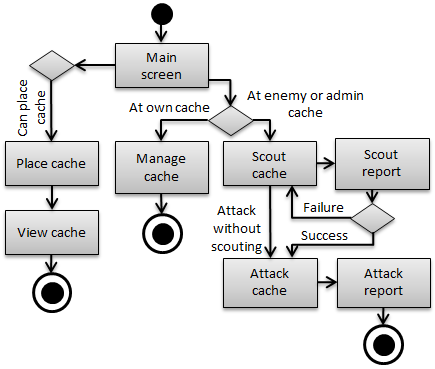
\includegraphics[width=0.5\textwidth]{images/key_actions}
	\caption{Screen map for key game actions.}
	\end{center}
	\vspace{-20pt}
\end{wrapfigure}

There are three main actions key to the game of Fortitude. They are creating caches (place cache), defending caches (manage cache) and conquering caches (scout then attack cache), and all are easily accessible through the main screen. Each action requires the user to be present at the cache/location of new cache, and the buttons calling these commands will be greyed out if this is not the case (see fig 2.2). The choice to combine both managing a cache the user owns – that is, depositing or withdrawing points in the cache to defend it against attack, or withdrawing all points to abandon the cache – and attacking an enemy cache into one ‘cache action’ button was taken to simplify the process of playing the game for the user while at the same time reducing redundancy and clutter on the main screen.

\subsection{Viewing caches}

\begin{wrapfigure}{l}{0.5\textwidth}
	\vspace{-20pt}
	\begin{center}
	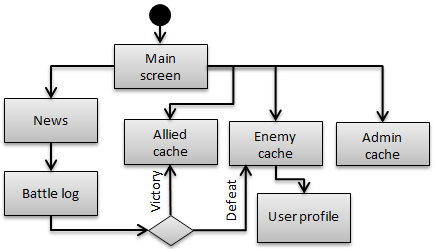
\includegraphics[width=0.5\textwidth]{images/viewing_caches}
	\caption{Screen map for key game actions.}
	\end{center}
	\vspace{-20pt}
\end{wrapfigure}
The ability to view caches is also integral to the above three actions, and is available at all times from the main screen (see fig 2.15) – the user does not have to be present at a cache to view its details. This is to enable the user to plan their game strategy, and keep track of their caches, and includes an option for the user to plan a route to the cache (functional requirement 5.3.4 Path finding) which will display on the map on the main screen (see fig 2.14). Beyond this, no game functions can be performed from viewing a cache – this must be done through the cache action button when physically present at the cache. However, the user profile of an enemy cache’s owner can be viewed, and caches can be reported to admins (see 2.2.5).

The user is also taken to view a cache after another player has attacked one of their caches. The user will be taken to the cache in question; if their defenders were victorious, they will see an allied cache, but if the attackers won they will see an enemy cache.

\subsection{Reading and sending messages}
\begin{wrapfigure}{l}{0.5\textwidth}
	\vspace{-20pt}
	\begin{center}
	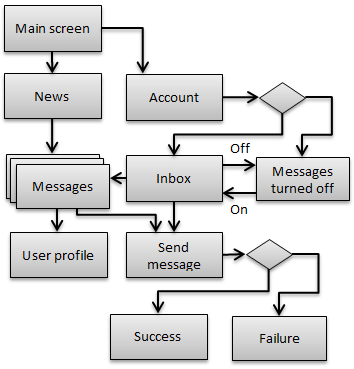
\includegraphics[width=0.5\textwidth]{images/sending_messages}
	\caption{Screen map for key game actions.}
	\end{center}
	\vspace{-20pt}
\end{wrapfigure}
The primary way that users interact with other users other than directly attacking their caches is by sending messages. This allows users to form alliances and build complex battle strategies within the game and satisfies requirement 5.4.1: User communication. From the inbox, users are also given the option to turn the messaging system off if they do not wish to use it. When sending a message, the user will be informed through a ‘Failure’ screen if the recipient has messages turned off – or if an error prevented the message being sent. This is to ensure the user is kept informed about their actions and does not send multiple messages believing the previous ones to have failed. Users are also given the chance to report communications or block users if they wish to (see 2.2.5).

\subsection{Reporting and Blocking}
\begin{wrapfigure}{r}{0.25\textwidth}
	\vspace{-20pt}
	\begin{center}
	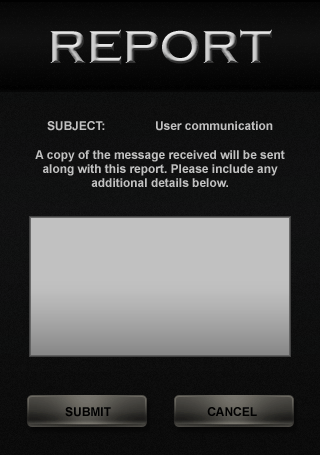
\includegraphics[width=0.25\textwidth]{images/report_mockup}
	\caption{Screen map for key game actions.}
	\end{center}
	\vspace{-20pt}
\end{wrapfigure}
Requirements 5.2.2: Cache reporting and 5.4.2: Communication reporting both require the user to be able to alert the administrators of certain caches or communications. This is anticipated to include a cache placed on a private or otherwise inaccessible location, or users behaving inappropriately towards others, and will be handled through a single report form (fig 2.8). The subject line of the report form is automatically filled in according to the screen from which the user decided to report (see fig 2.9), and a copy of the offending message, user profile or cache is sent along with the message to give administrators as much information as possible.

\begin{wrapfigure}{l}{0.5\textwidth}
	\vspace{-20pt}
	\begin{center}
	\begin{tabular}{| p{0.22\textwidth} | p{0.68\textwidth} |}
		\hline
		Outlaw camp
Enemy cache
Allied cache
Message
User profile
 &
		Outlaw camp
User owned cache
User owned cache
User communication
User profile
 \\
		\hline
	\end{tabular}
	\caption{Screen map for key game actions.}
	\end{center}
	\vspace{-20pt}
\end{wrapfigure}

Blocking users ensures that a user will receive no messages from the user they have blocked, though both users will be able to view and attack each other’s caches. Users can view a list of blocked users from their inbox, and from here can block or unblock a user. Blocking a user can  also be done from the user profile.

\subsection{Administrators acting on user request}

\subsection{Reporting and Blocking}
\begin{wrapfigure}{l}{0.5\textwidth}
	\vspace{-20pt}
	\begin{center}
	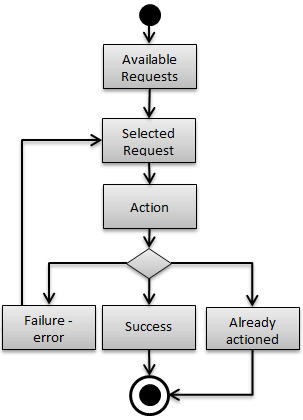
\includegraphics[width=0.5\textwidth]{images/admins_acting}
	\caption{Screen map for key game actions.}
	\end{center}
	\vspace{-20pt}
\end{wrapfigure}

User requests submitted from the application are always in the form of a report, as detailed above in 2.2.5. However, a user may submit other requests through the website, including a request to delete their account or a support question sent through the help page. All of these requests must be acted upon by an administrator; this is done through the admin section of the website. Certain requests, such as deleting the account, must be confirmed by the user before they are sent to the administrator; this is done by an email being sent to the user after they have initiated the request. The email contains a link to confirm the request; clicking on this link generates a request for the administrators to action.

Here, administrators are able to see a page of all available requests, a request being available if it is not being worked on by another administrator at the time. The administrator selects a request (thereby removing it from the available requests page visible to all admins) and performs an action on it, which may be to complete the request or to flag the request if it cannot be completed at that point or by that administrator. The administrator will be informed of the result of their action and any details about a failure, such that the administrator can correct their mistake or flag the request. In the unlikely instance that two administrators try to action the same request (although occurrences of this are minimised by the request being removed from the available requests page), the first action will be performed and the second administrator informed of this when they submit their own action. Once acted upon, requests will be accessible through a ‘past requests’ page.

\subsection{Miscellaneous other}

\subsection{Reporting and Blocking}
\begin{wrapfigure}{l}{0.25\textwidth}
	\vspace{-20pt}
	\begin{center}
	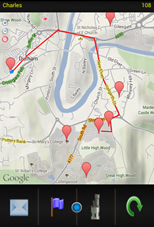
\includegraphics[width=0.25\textwidth]{images/route_mapping}
	\caption{Screen map for key game actions.}
	\end{center}
	\vspace{-20pt}
\end{wrapfigure}

Signing out is done from the user account settings, accessed from clicking on the status bar on the main screen.

Special placement caches are not available by user request; they will appear on the screen if the user has the application open while at the correct location. The user will at this point be asked to accept or reject the reward for finding the cache, without having to conquer the cache to receive it.

Routes to caches are shown on the main map as a thick red line (see fig 2.14). They can be planned from any type of ‘view cache’ screen and are cleared through the account menu. Routes are also cleared before each route is mapped, such that there can only be one route displaying on the map at any given time.


\section{User Interface Design – Fortitude Application}

\subsection{Main screen}


The main screen is the core of the Fortitude application through which all key features are easily accessible. These are split into features relating to playing the game, grouped in the action bar at the bottom of the screen, and features relating to providing the user with information or allowing them to access their account, grouped in the status bar at the top of the screen. When clicked, this status bar leads the user to their account menu through which they can sign out, access their message inbox, or view the help screen. The status bar also displays the point balance available to the user; as points are required for every action, it is important that this information is very visible, as specified by functional requirement 5.2.1: Account balance.

The action buttons relating to game play are grouped at the bottom of the screen, where it is most ergonomic for the user to access them. Each button is clearly distinct and, where appropriate, contains easily discernible extra information – such as the place cache and cache action buttons being greyed out when unavailable (see fig 2.2) and the recent news having a notification symbol to indicate unread news (fig 2.16). 

The main area of the home screen is the map, chosen as a very user friendly interface for the game and fulfilling several requirements including 5.3.1: Display location and 5.2.3: Nearby caches. Caches are clearly distinguished with different coloured pins to differentiate between admin, allied and enemy caches, as per requirement 5.2.3: Cache ownership and 5.2.26: Distinguishing cache owners; the colours are chosen to account for those with colour blindness (see fig 2.17). The map itself is controlled with the touch screen, using swipe or drag to navigate and pinch to zoom (zoom required by 5.3.3: Map zooming). To reduce data usage as per non-functional requirement 5.2.30: Data usage, adjusting the map view by zoom or location will not load the caches for that area of the map. This will be done by the green refresh arrow on the right of the status bar which also updates point balance and recent news feed as required.

\subsection{Unactivated main screen}

The main screen for the unactived user is identical in appearance to the main screen for an activated user (see fig 2.15), with the only difference being in the bottom bar. On the standard main screen this contains several buttons linking to features or actions which are not available to unactivated users – as specified by functional requirement 5.1.2: Account Activation. Here, this bar is replaced by a banner reminding users to activate their account; when clicked, this banner leads to the resend activation email page.

All other features have the same functionality as the main screen. The only difference is in navigating the map; on the unactivated account, each request to load a new view of the map also loads every cache within that view. This is because the unactivated user is not able to refresh the screen, as this button is located on the action bar which is not available here.

\subsection{User text input}

Many screens make use of text the user has input, most notably those involved with signing in or creating a new account (see fig 2.7) as well as sending messages to users (fig 2.19) or reports to administrators. Text input is handled through the on screen keyboard that is standard on an android phone (see fig 2.20). 

Should the user input invalid information, such as incorrect login details, then an error message will be displayed (see fig 2.21). The screen behind this message will be dimmed to ensure the message is clearly visible. A similar design will be used for all message alerts to the user, such as error messages, status messages (for example ‘connecting to server’) or confirmation messages, which may have two options for the user to choose between (see fig 2.22)

Message boxes and text input fields are always of a consistent design to make them easy for the user to identify, though message boxes may stretch to contain longer messages.

\subsection{Menu and Information screens}

Many screens in the application give the user a set of options or provide some form of information. Viewing caches is one such example, as is the account menu (fig 2.23). The primary aim of these screens is to make the information as clear as possible to the users while at the same time making efficient use of space, so that the user does not have to click through multiple nested menus to access any feature. There is also consistency across screens; the ‘cancel’ button, for example, is always either the central bottom button or the bottom right.

The use of images when viewing a cache provides not only aesthetic appeal, but also serves a functional purpose. With different images used for enemy caches, allied caches and administrator caches, it is easy to identify from the cache screen what type of cache is being viewed; again, this refers back to requirement 5.2.26: Distinguishing caches.

\subsection{List screens}

Lists are used for displaying news items and messages in the inbox. Each screen displays several items on a single screen with forward and back buttons at the bottom of the screen to view the next page of items. This helps to limit data usage and loading times for the user whilst also providing an easy to navigate, well ordered system of displaying the items.

The use of icons to distinguish between types of items – battle reports and news icons, for example – makes it easier to take the list as a whole in without difficulty, and fading the icons of items which are not new helps the user find the important information with greater ease (as shown in the bottom 3 icons of fig 2.25).

\subsection{Action screens}

Screens involving direct interaction with caches, such as attacking, managing (withdrawing or depositing soldiers) or placing caches are of a similar layout to provide consistency throughout the game. The screens are clearly differentiated by the use of different images – such as a charging soldier on the attack screen versus a sneaking soldier on the scouting screen (see figs 2.26 and 2.27) as well as by the action title being clearly displayed. The name of the cache involved is also clearly displayed on the screen. Any time that user input is required in these screens it is done in such a way to restrict the values of possible user input to those which are known to be valid, such as using a slider to change the number of soldiers committed to an action or choosing between a choice of names when creating a cache (see fig 2.28). This is to make the process of game play as quick and error free as possible.

\subsection{Reporting results}

Any action with an unknown outcome is reported to the user using a screen of the same design, again to make the app consistent and increase the user’s familiarity with how it works and where information is displayed. Where relevant, the image of the report screen reflects the outcome – such as a scroll for a successful scouting mission versus a tomb stone for a failed one (fig 2.29). As ever, this is both for aesthetic reasons and to communicate the necessary information to the reader clearly and quickly.

A similar report screen is also accessible from the news feed for the report of a cache the user owns which has been attacked by another player. This screen differs in that the name of the cache is more prominent and there is a link to view the cache on the map; this is required to identify the cache as the user may not be present at the cache’s location.

\subsection{Static screen}

The final type of screen is a static screen. This is one not designed for much user interaction; the full screen is comprised of a single image or static text, such as the Fortitude logo on the splash screen or the help screens (fig 2.1). The splash screen itself has no buttons for the user to progress, as the app will automatically move on once it has loaded. Other static screens, such as the help screens, have a button to move on from this screen.

Static screens are used for errors which cause the app itself to be unplayable – the most common of which would be the user not having internet connection available (see fig 2.31) – and the user will be unable to move from this screen until the error has resolved. A static screen is also used for when a user comes across a special placement cache, with which they cannot interact but must either accept or reject the prize.

With the exception of the help screens, static screens cannot be called by the user; they are initiated by the server and used to send a message to the user that cannot be ignored or minimised until the server allows and normal game play can resume.

2.4	User Interface Design – Fortitude-game.co.uk}

\subsection{Site Layout}

The visual design of the website was chosen to reflect the dramatic battle-driven nature of the game of Fortitude. It clearly echoes the app in its sombre colour scheme of black, white and greys, and the use of the two flags image used as Fortitude’s logo (see fig 2.4). The choice of a more serious design both in the website and the app is to reflect the strategic and ‘epic’ style of game that Fortitude is, appealing to players of all ages.

The basic structure of the website is for the page to be divided into three, with the top area containing navigation (including administrator links), the sidebar to the left containing key information and the larger area to the right displaying the page content for each page (see fig 2.32). Both the sidebar to the left and the main page content use modules to display content, making the information easily and quickly accessible. The administration links have been placed above the main page to ensure that they cannot interfere with the usual page content but are not sidelined and hard to get to; it is anticipated that administrators would mainly use the website for admin purposes, and so need the links to be clearly visible. These links will not be displayed for any user who is not an administrator; should they reach an administrator page, they will be shown a 404 page. Similarly, some pages are restricted to users; should a visitor who is not logged in attempt to view a page such as the account page, they will be redirected to the login/sign up screen.

The use of drop down sub menus is important to increase ease of navigation, enabling users to quickly reach areas of the website without over cluttering the top bar itself. However, as not all devices have a hover feature (such as tablets or phones), no area of the website will only be accessible through these sub menus.

\subsection{Site Content}

The content of the website will in many cases mimic that of the app, though in greater depth or with greater functionality – for example, the user can view caches on a map as they can through the phone, but can also apply a filter to display only their own or only enemy caches, as per requirement 5.4.7: Overview Map (see fig 2.33). In addition, some functionality is only available through the website – such as the ability to search for a user or cache by name, or the ability to view an activity log of recent activity associated with that account, specified in requirement 5.3.6: Activity Recording. Certain content, such as the home screen and site news, is visible to all whether logged in or not so as to give potential users a feel for the game and encourage them to sign up and participate. Other areas will redirect the user to the Login page which consists of two modules, one to log in and one to sign up. These modules will also be visible on the side bar at all times unless the user is logged in, in which case the side bar will display key information.

\subsection{The Map}

The map will use the familiar google maps interface with zoom, street view, and different types of map (satellite, terrain etc). The user can search the map by location, username (ie all caches owned by a certain user) or cache name; should multiple caches with the same name be found, both would be displayed on the map (and the zoom adjusted until both were visible), and the user could zoom in on the correct one. The option to filter caches is done through a drop down menu with filters including ‘All caches’, ‘My caches’, ‘Enemy caches’, and ‘Outlaw camps’ (non-player caches). Updating the map by either filtering or searching is done asynchronously, providing a much smoother experience for the user without having to reload the page each time a request is sent. Different types of caches are distinguished as on the app by colour and the presence of a dot, such that colour blind people can also tell caches apart. A cache displays its name and, when clicked on, choices to view the cache details or plan a route to it; this option will bring up a dialogue box asking for the location to plan the route from.

\subsection{Sidebar}

As mentioned previously in the Design Methodology (2.1.2), users will in future be able to personalise sections of the website including the sidebar to display the modules most appropriate to them. Until such a point, the sidebar will display to a logged in user a search bar, an account summary, a list of the user’s five most active caches – determined by the cache with the greatest frequency of events in its history – and a list of the user’s five most recent events. If a user who is not logged in views the site, the sidebar will contain the search module as well as modules to log in or sign up.

The title ‘Elite Warlord’ in fig 2.34 Corresponds to the user’s level, determined by the number of caches they own. The avatar and user title serve little purpose as far as game play is concerned, but contribute towards personalising a user’s account and, in the levels, giving a tangible goal to aim for in the game.

\subsection{Administrator pages}

The administrator features of the website are accessible through the navigation links at the top of the screen, which are only visible to users logged in as administrators. These are highlighted in green, the colour making them stand out and separate from the rest of the website. The tasks that can be completed from each page are shown below in fig 2.36. 

Caches	View all caches, grouped under ‘user cache’ and ‘outlaw cache’. Includes options to view the history of or delete caches of any kind or add outlaw caches, as well as managing or editing outlaw caches.
Users	View the entire user list. Includes options to send users an official warning or other communication and to remove a user account (this would only be done by user request).
Reports	View all user requests that need to be acted on, and select individual requests to action.
Special Placement	Create and manage special placement caches.
Announcements	Post an announcement to the site (appears on the home page and news), and edit or delete old announcements.

\subsection{Tasks carried out by admins from each administrator page.}

Administrator pages can be roughly grouped into two types; those that involve viewing a database, and those that involve creating data such as a cache, special placement or announcement. Database style pages are laid out as shown in fig 2.37 (the header and sidebar sections are not shown, but are the same as the rest of the site). Filtering the database and commands such as creating new caches or, on the user request page, viewing past requests are linked from the top of the page for easy access, and the database is grouped by a tab system into the types of database. This avoids having redundant fields in an entry – such as the ‘owner’ field for an outlaw camp entry. The administrator cannot ever see the whole database on one page; they are originally shown only the filter section and must access the database by running a query from here. Should the query be too large, the administrator will be requested to narrow down the filter.

Creating data is handled through a form interface which, despite its simple design, is arguably the best method of data input for users (Dix, Finlay et al, 1993: PAGE NUMBER). The form provides user feedback for incorrect or invalid data entries in the same way as creating a user account would (see section 2.1.2).



\begin{tabular}{| p{0.22\textwidth} | p{0.68\textwidth} |}
	\hline
	Caches &
	\lipsum[1] \\
	\hline
	Users &
	\lipsum[2] \\
	\hline
\end{tabular}
